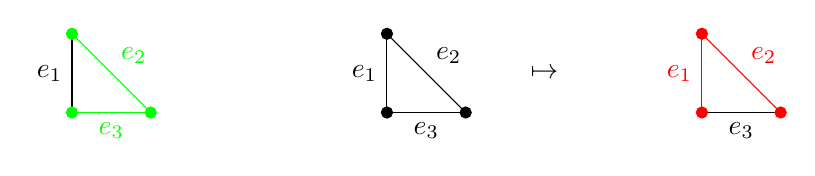
\begin{tikzpicture}

    \begin{scope}[xshift = -4 cm]
        
        \coordinate (v_1) at (0, 0);
        \coordinate (v_2) at (1, 0);
        \coordinate (v_3) at (0, 1);

        \draw [color = green] (v_1) -- node [below]       {$e_3$} (v_2);
        \draw [color = green] (v_2) -- node [above right] {$e_2$} (v_3);
        \draw [color = black] (v_3) -- node [left]        {$e_1$} (v_1);

        \filldraw [color = green] (v_1) circle (2pt);
        \filldraw [color = green] (v_2) circle (2pt);
        \filldraw [color = green] (v_3) circle (2pt);

    \end{scope}

    \draw (-2, 0.5) node {$\mapsfrom$};

    \begin{scope}
        
        \coordinate (v_1) at (0, 0);
        \coordinate (v_2) at (1, 0);
        \coordinate (v_3) at (0, 1);

        \draw [color = black] (v_1) -- node [below]       {$e_3$} (v_2);
        \draw [color = black] (v_2) -- node [above right] {$e_2$} (v_3);
        \draw [color = black] (v_3) -- node [left]        {$e_1$} (v_1);

        \filldraw [color = black] (v_1) circle (2pt);
        \filldraw [color = black] (v_2) circle (2pt);
        \filldraw [color = black] (v_3) circle (2pt);

    \end{scope}

    \draw (2, 0.5) node {$\mapsto$};

    \begin{scope}[xshift = 4 cm]
        
        \coordinate (v_1) at (0, 0);
        \coordinate (v_2) at (1, 0);
        \coordinate (v_3) at (0, 1);

        \draw [color = black] (v_1) -- node [below]       {$e_3$} (v_2);
        \draw [color = red]   (v_2) -- node [above right] {$e_2$} (v_3);
        \draw [color = red]   (v_3) -- node [left]        {$e_1$} (v_1);

        \filldraw [color = red] (v_1) circle (2pt);
        \filldraw [color = red] (v_2) circle (2pt);
        \filldraw [color = red] (v_3) circle (2pt);

    \end{scope}

\end{tikzpicture}